\documentclass[margin = 10pt]{standalone}
\usepackage{tikz,pgfplots}
\usetikzlibrary{calc}
\usepgfplotslibrary{groupplots}
\pgfplotsset{%
    compat = 1.18,
    every axis title/.style ={
            align=left,
            fill=blue!20,
            minimum width=4cm,
            text = black,
            rounded corners=1pt,
            font = \large,
            line width =0.1pt,
            anchor=east,
            at={($(axis description cs:0,0.85)+(-1cm,0)$)},
        },
    }%

\begin{document}
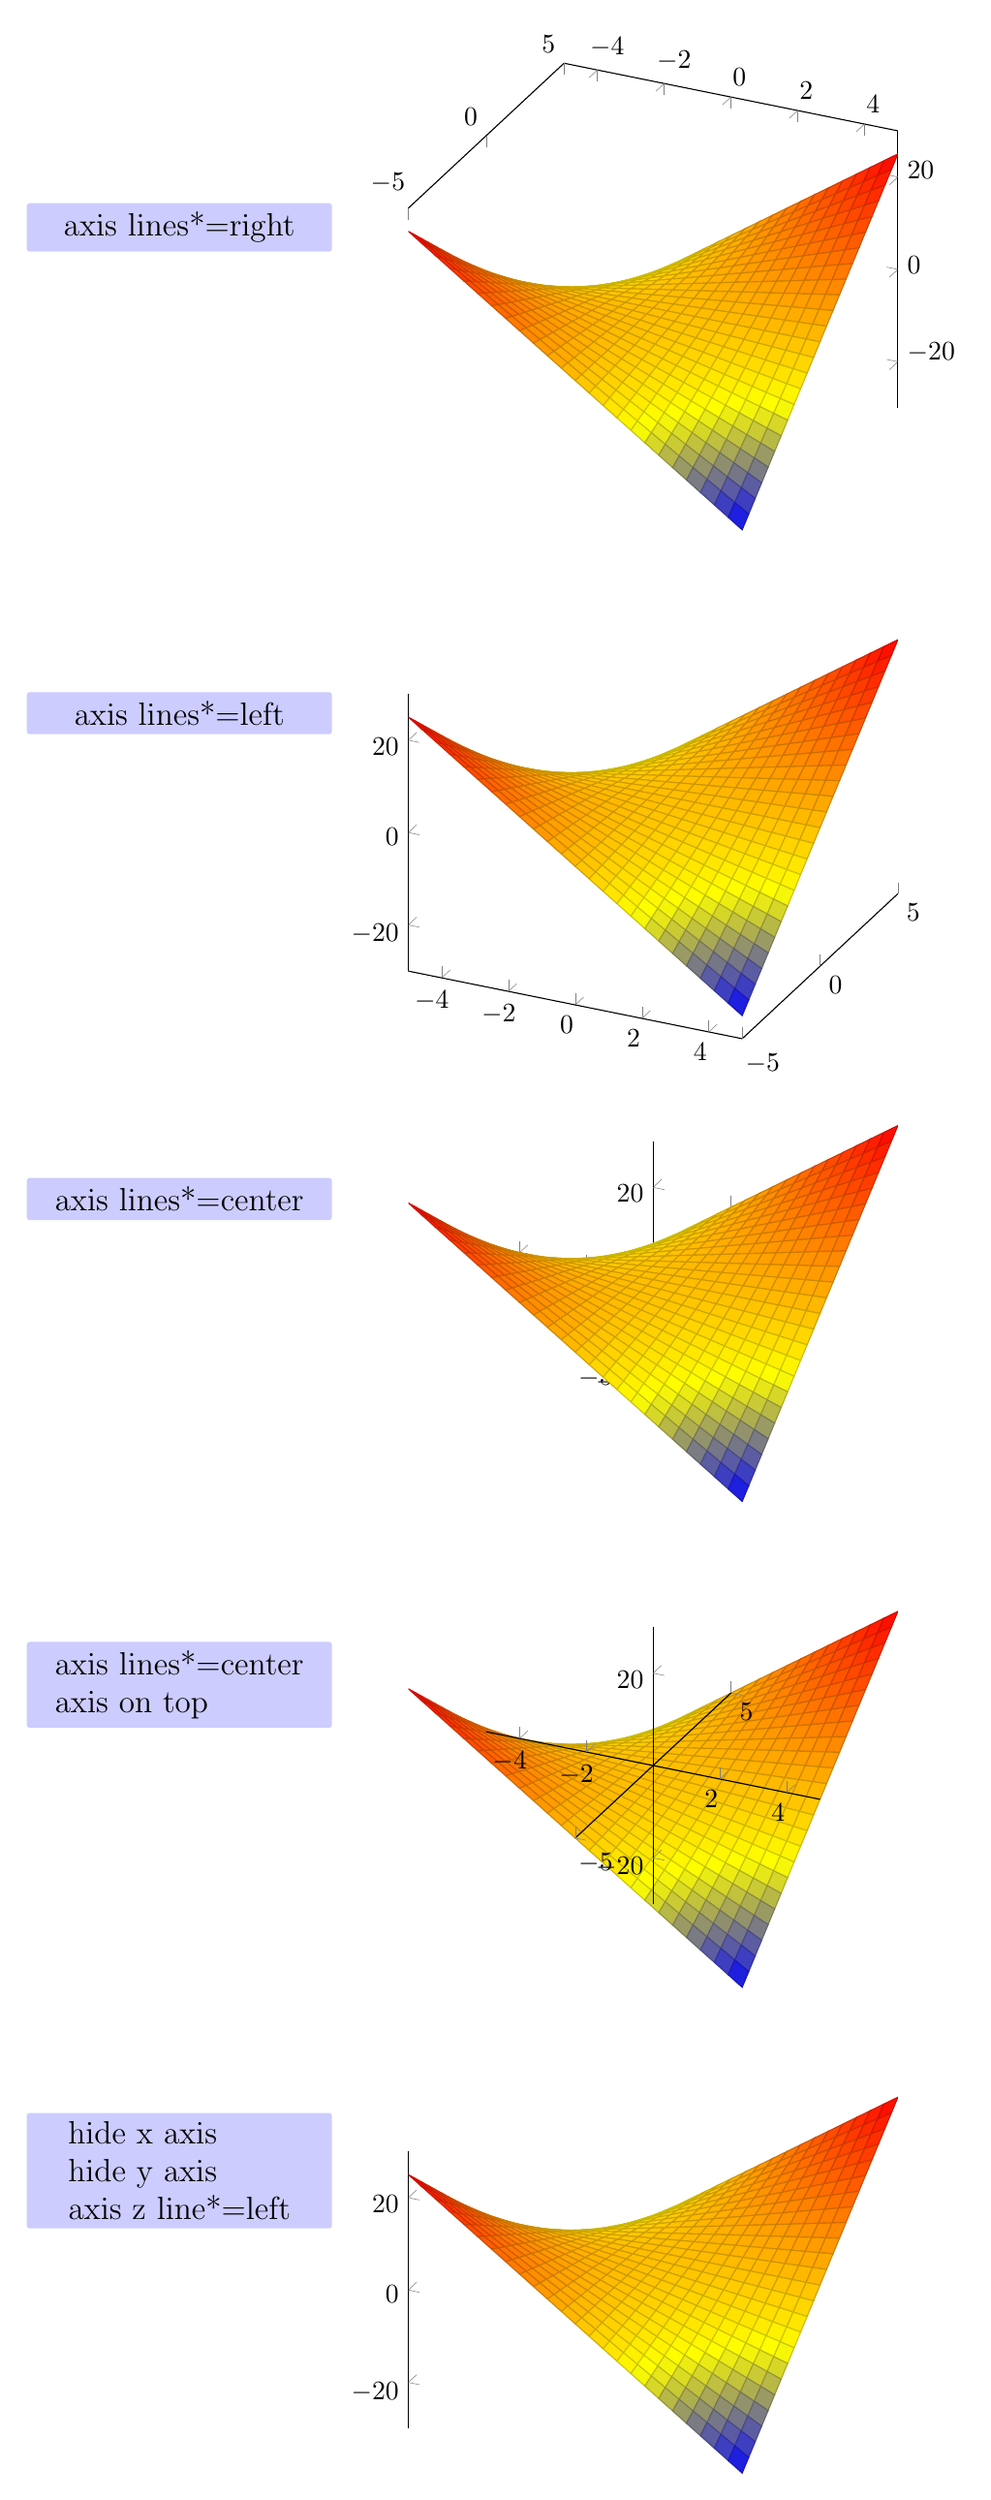
\begin{tikzpicture}
\begin{groupplot}[
    group style={
        group size=1 by 5,vertical sep=-0.05cm,
        },width=8cm,height=8cm,
    ]
    
\nextgroupplot[
    title = {axis lines*=right},
    axis lines*=right,
    ] \addplot3 [surf] {x*y};
    
 
\nextgroupplot[
    title = {axis lines*=left},
    axis lines*=left
    ] \addplot3 [surf] {x*y};

    
\nextgroupplot[
    title = {axis lines*=center},
    axis lines*=center,
    ] \addplot3 [surf] {x*y};
    
    
\nextgroupplot[
    title = {axis lines*=center\\ axis on top},
    axis lines*=center,
    axis on top
    ] \addplot3 [surf] {x*y};

    
\nextgroupplot[
    title = {hide x axis\\ hide y axis\\ axis z line*=left},
    hide x axis,
    hide y axis,
    axis z line*=left
    ] \addplot3 [surf] {x*y};



\end{groupplot}
\end{tikzpicture}



 



% \begin{axis}[
%     name= r3,
%     anchor = north,
%         at={($(r2.south)+(0cm,-2cm)$)},
%     title = {hide x axis\\ hide y axis\\ axis z line*=left},
%     hide x axis,
%     hide y axis,
%     axis z line*=left,
%     ]
% \addplot3 [surf] {x*y};
% \end{axis}

% \begin{axis}[
%     anchor = west,    
%     at={($(r3.east)+(2cm,0)$)},
%     title = {hide axis},
%     hide axis
%     ]
% \addplot3 [surf] {x*y};
% \end{axis}





% \begin{axis}[
%     name= r4,
%     anchor = north,
%         at={($(r3.south)+(0cm,-2cm)$)},
%     title = {hide x axis},
%     ]
% \addplot3 [surf] {x*y};
% \end{axis}

% \begin{axis}[
%     anchor = west,    
%     at={($(r4.east)+(2cm,0)$)},
%     title = {hide axis},
%     hide axis
%     ]
% \addplot3 [surf] {x*y};
% \end{axis}








% \end{tikzpicture}







































% \begin{tikzpicture}[remember picture]
% \begin{axis}[
%     % 3d box=complete,
%     3d box=background,
%     grid,
%     % box | top | middle | center | bottom | none | left | right
%     % 带* 没有箭头
%     % axis lines=center,
%     % axis lines*=right,
%     % 位置
%     axis x line* = box,
%     % axis y line = center, 
%     % axis z line = center, 
%     % hide axis = true,
%     % axis on top,
%     % 方向
%     % y dir = reverse,
%     % x dir = reverse,
%     % 偏移
%     % axis line shift = 3pt,
%     % axis x line shift = 30pt,
%     % 
%     % 设置轴刻度的跳跃值 crunch | parallel | none 
%     axis x discontinuity = crunch ,
%     xtick={-0.4,0,4},
%     % axis y discontinuity = parallel ,
%     x axis line style = {-latex[],red},
%     % y axis line style = {-latex[],blue},
%     % axis line style = {-Latex[],red},
%     ]
    
    
% \addplot3 [smooth,surf] {exp(-x^2-y^2)*x};
% \end{axis}
% \end{tikzpicture}
\end{document}